\chapter{Первая глава}

\section{Вступление}

Типичное оформление рисунка.

\begin{figure}[ht]
    \centering
        \begin{subfigure}[b]{0.3\textwidth}    
        \centering
            $$\begin{array}{l}
            F \to x \;|\; y \;|\; (S) \\
            T \to F \;|\; T \ast F \\
            S \to T \;|\; S + T \\    
            \end{array}$$
            \caption{}
        \end{subfigure} %    
        \begin{subfigure}[b]{0.6\textwidth}
        \centering
            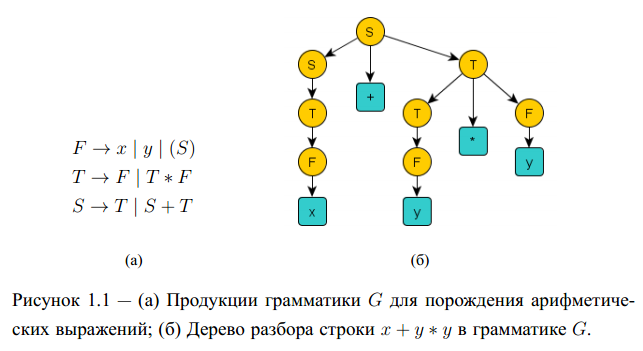
\includegraphics[scale=0.7]{parseTree.png}
            \caption{}
        \end{subfigure}
     
        \caption{(a) Продукции грамматики $G$ для порождения арифметических выражений; 
                 (б) Дерево разбора строки $x+y\ast y$ в грамматике $G$.}
        \label{fig_parsetree}
\end{figure}

\clearpage
Типичное оформление таблицы.

\begin{table}[ht]
    \caption{Расчет весомости параметров ПП}
    \label{tab_weight}
    \centering
        \begin{tabular}{|c|c|c|c|c|c|c|c|c|}
        \hline \multirow{2}{*}{Параметр $x_i$} & \multicolumn{4}{c|}{Параметр $x_j$} & 
            \multicolumn{2}{c|}{Первый шаг} & \multicolumn{2}{c|}{Второй шаг} \\
        \cline{2-9} & $X_1$ & $X_2$ & $X_3$ & $X_4$ & $w_i$ & 
            ${K_\text{в}}_i$ & $w_i$ & ${K_\text{в}}_i$ \\
        \hline $X_1$ & 1 & 1 & 1.5 & 1.5 & 5 & 0.31 & 19 & 0.32 \\
        \hline $X_2$ & 1 & 1 & 1.5 & 1.5 & 5 & 0.31 & 19 & 0.32 \\
        \hline $X_3$ & 0.5 & 0.5 & 1 & 0.5 & 2.5 & 0.16 & 9.25 & 0.16 \\
        \hline $X_4$ & 0.5 & 0.5 & 1.5 & 1 & 3.5 & 0.22 & 12.25 & 0.20 \\
        \hline \multicolumn{5}{|c|}{Итого:} & 16 & 1 & 59.5 & 1 \\
        \hline
        \end{tabular}
\end{table}

Список:
\begin{itemize}
\item слово «Стр.» над колонкой с номерами страниц;
\item выделение глав жирным шрифтом и верхнем регистром (и предварительным «Глава N»);
\item включение в оглавление специальных разделов («Вступление», «Список сокращений», «Выводы», «Список литературы»...) на уровне обычных глав, но без слова «Глава» и нумерации;
\item включение в оглавление подразделов и пунктов, но не подпунктов и ниже;
\item и разнообразные красивые выравнивания.
\end{itemize}

Ссылка на литературу: см. \cite{Кнорринг1976}.
